\documentclass{article}
\usepackage[utf8]{inputenc}
\usepackage{amsmath}
\usepackage{graphicx}
\usepackage{float}

\title{COMP6245 : Lab 1 Report}
\author{Thanakorn Panyapiang(31446612)}

\begin{document}

\maketitle
\section{Linear Algebra}
The command U @ U.T produces a 3x3 identity matrix because of a symmetric property of B. \\
\indent Since B is a symmetric matrix, all eigenvectors of B are othorgonal to each other. Therefore, U,a matrix which each column represents a unit eigenvector of B(according to numpy specification), is an \textit{orthorgonal matrix}.

One property of an orthorgonal matrix is $A^T = A^{-1}$. Substituing this in the the command will get the result as follow:
\[U(U^T) = U(U^{-1})\]
\[U(U^{-1}) = I \] 

\maketitle
\section{Random Numbers and Univariate Distributions}
The distribution of uniform random samples for different numbers of samples and bins is as follow
\begin{center}
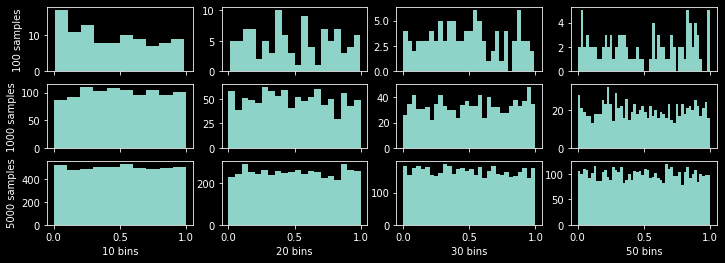
\includegraphics[scale=0.5]{uniform_random_numbers}
\end{center}
It can be observed that, when the number of samples is high, data is distributed equally regardless of the number of bins which causes the variation within bin counts to be low.

For samples drawn from a Gaussian distribution, the density of data, regardless of the number of samples, is higher when the value is close to mean and most of the data is located within 2 standard deviation(-2 to 2).
\begin{center}
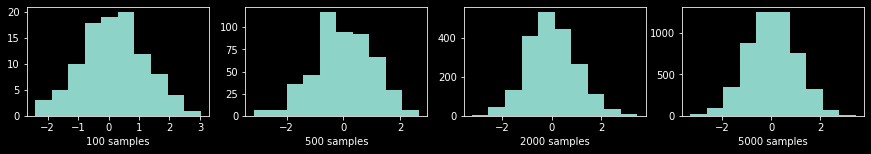
\includegraphics[scale=0.4]{gaussian_random_numbers}
\end{center}

In the last samples where a data is generated by summation of uniform random numbers, the distribution of data is similar to the samples drawn from a Gaussian distribution.
\begin{center}
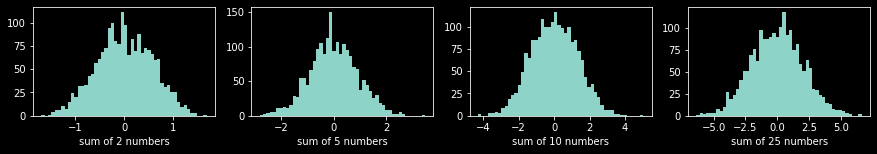
\includegraphics[scale=0.4]{sum_random_numbers}
\end{center}

\maketitle
\section{Uncertainty in Estimation}

\maketitle
\section{Bivariate Gaussian Distribution}

\maketitle
\section{Sampling for Multivariate Gaussian Distribution}
Data in X is normally distributed with mean = 0 and standard deviation = 1 for both two random variables. This can be observed by the density of data increase when the value come close to 0 and the majority of data is located within 2 standard deviation(-2 to 2).

For Y, although the data also has a normal distribution, the distribution in X-axis is wider than X due to the linear transformation which is performed on X that cause the variance of one random variable to be higher.

\maketitle
\section{Distribution of Projections}
\end{document}